\chapter{श्वसन क्या है?}\label{ch:g7:what-is-respiration}

किसी बंद मरतबान में एक कठ-जूँ रखो और घंटों बाद उस मरतबान की हवा बदल चुकी
होती है: उसकी कुछ \omterm{def:g7:what-is-respiration:respiration}{ऑक्सीजन} जा चुकी है और उसकी जगह \omterm{def:g7:what-is-respiration:respiration}{कार्बन डाइऑक्साइड} आ गई
है। यही अंकुरित होते \omterm{def:g2:from-seed-to-plant:seed}{बीज}, किसी कुकुरमुत्ते, किसी सुनहरी मछली, या जीवित
\omterm{def:g6:decomposers-and-soil:soil}{मिट्टी} के एक चम्मच के साथ दोहराओ --- हर बार वही नतीजा।
\Cref{prop:g4:breathing:exchange} ने यह अदला-बदली तुम्हारी अपनी छाती में
दिखाई थी; और यह साल इस विचार को उसकी पूरी चौड़ाई में खोलता है: यह
अदला-बदली मनुष्य की आदत नहीं, ख़ुद जीवन की एक ख़ासियत है।

\section{श्वसन, परिभाषित और नापा हुआ}

\begin{definition}[श्वसन]\label{def:g7:what-is-respiration:respiration}
\emph{श्वसन}\index{श्वसन} वह गैस-विनिमय है जिससे कोई \omterm{def:g6:exploring-our-environment:components}{सजीव} अपने आस-पास से
\emph{ऑक्सीजन}\index{ऑक्सीजन} लेता है और \emph{कार्बन
डाइऑक्साइड}\index{कार्बन डाइऑक्साइड} छोड़ता है। इसे
\emph{श्वासोच्छ्वास}\index{श्वासोच्छ्वास} से नहीं गड्डमड्ड करना चाहिए,
यानी \cref{def:g4:breathing:movements} वाली छाती की दिखती गतियों से:
श्वासोच्छ्वास श्वसन की \emph{सेवा} करने का एक तरीक़ा भर है; और श्वसन
ख़ुद वह गैस-अदला-बदली है, जो हर जीवित \omterm{def:g5:first-look-at-cells:cell}{कोशिका} में चलती रहती है, गतियाँ
हों या न हों।
\end{definition}

\begin{proposition}[यह अदला-बदली कैसे दिखाई जाती है]\label{prop:g7:what-is-respiration:shown}
मेज़ पर की दो मानक जाँचें \omterm{def:g7:what-is-respiration:respiration}{श्वसन} को उघाड़ देती हैं:
\begin{itemize}
  \item किसी बंद पात्र में लगा \emph{ऑक्सीजन-मापक} दिखाता है कि भीतर
        बैठे \omterm{def:g6:exploring-our-environment:components}{सजीव} के रहते \omterm{def:g7:what-is-respiration:respiration}{ऑक्सीजन} का स्तर गिरता जाता है;
  \item और \emph{चूने का पानी}\index{चूने का पानी}, यानी वह साफ़ तरल जो
        \omterm{def:g7:what-is-respiration:respiration}{कार्बन डाइऑक्साइड} में दूधिया हो जाता है, तब धुँधला पड़ जाता है
        जब पात्र की हवा उसमें से गुज़ारी जाती है।
\end{itemize}
गिरती \omterm{def:g7:what-is-respiration:respiration}{ऑक्सीजन} और धुँधलाता \omterm{prop:g7:what-is-respiration:shown}{चूने का पानी}, और साथ में एक निर्जीव \omterm{met:g4:what-plants-need:fairtest}{नियंत्रण}
पात्र जो जितना का तितना बना रहे
(\cref{met:g4:what-plants-need:fairtest} --- न्यायी जाँच हर जगह हमारा
पीछा करती है): यही \omterm{def:g7:what-is-respiration:respiration}{श्वसन} है, नापा हुआ।
\end{proposition}
\admitted

\begin{example}[श्वसन करने वालों की नुमाइश]\label{ex:g7:what-is-respiration:gallery}
दोनों जाँचें एक पूरे चिड़ियाघर पर चलाओ: एक चूहा --- तेज़ गिरावट, जल्दी
धुँधलाहट; एक कठ-जूँ --- वही, पर छोटी; अंकुरित होते मटर --- साफ़-साफ़
(अंकुरित मटरों का मरतबान अपनी \omterm{def:g7:what-is-respiration:respiration}{ऑक्सीजन} एक दिन में ख़त्म कर सकता है); एक
कुकुरमुत्ता --- हाँ; तालाब के घोंघे --- हाँ; और जीवित \omterm{def:g6:decomposers-and-soil:soil}{मिट्टी} का एक
चम्मच --- हाँ, जिसके अरबों \omterm{def:g6:decomposers-and-soil:decomposers}{अपघटक} साथ-साथ \omterm{def:g7:what-is-respiration:respiration}{श्वसन} कर रहे हैं
(\cref{ex:g6:decomposers-and-soil:handful})। सिर्फ़ \omterm{met:g4:what-plants-need:fairtest}{नियंत्रण} मरतबान ---
कंकड़, सूखी बालू --- कुछ नहीं बदलता।
\end{example}

\begin{omfigure}
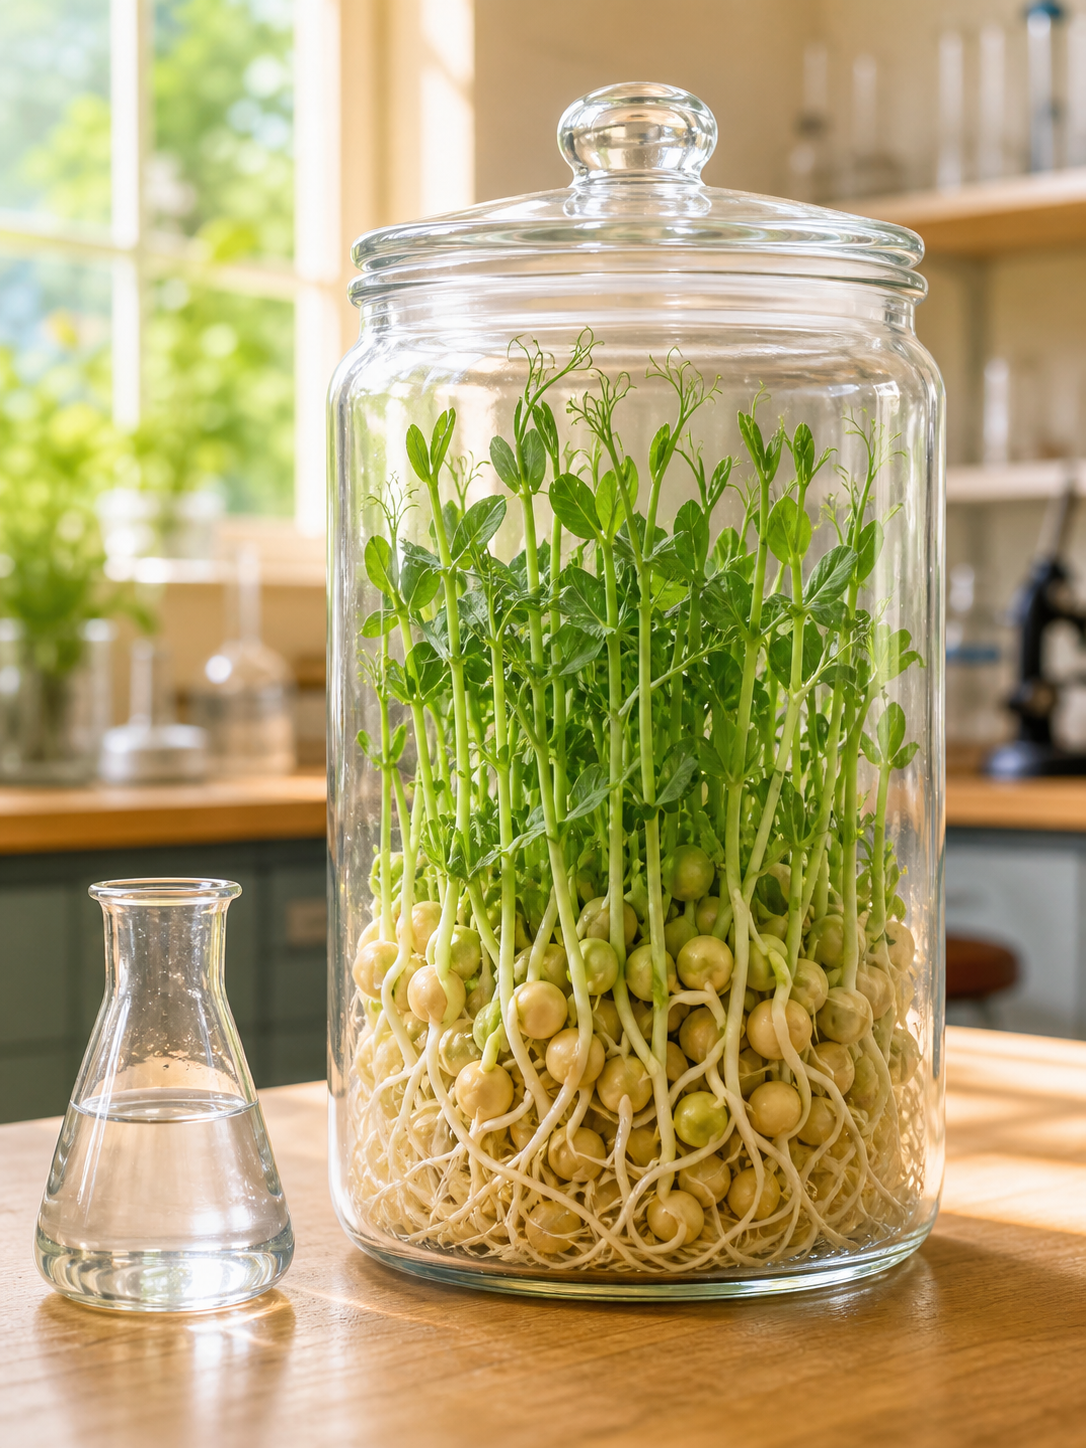
\includegraphics[width=0.46\linewidth]{images/book1/ai/g7-resp-peajar.png}

{\small मेज़ पर सबसे मामूली दिखने वाला \omterm{def:g7:what-is-respiration:respiration}{श्वसन} करने वाला: अंकुरित मटरों का
मरतबान अपनी \omterm{def:g7:what-is-respiration:respiration}{ऑक्सीजन} एक दिन में ख़त्म कर सकता है।}
\end{omfigure}

\begin{remark}[पौधे भी श्वसन करते हैं]\label{rem:g7:what-is-respiration:plants}
\Cref{rem:g6:plants-are-producers:gas} ने चलते-चलते यह कहा था; और
मरतबान इसे साबित कर देता है: गमले का \omterm{def:g1:plants-around-us:plant}{पौधा} \emph{अँधेरे में} अपने मरतबान
की \omterm{def:g7:what-is-respiration:respiration}{ऑक्सीजन} घटा देता है और चूने के पानी को किसी भी \omterm{def:g1:animals-around-us:animal}{जंतु} की तरह धुँधला कर
देता है। दिन के उजाले में \omterm{def:g5:food-webs:roles}{उत्पादकों} का निर्माण इस असर को ढक देता है ---
क्योंकि वह \omterm{def:g7:what-is-respiration:respiration}{श्वसन} के छोड़े से कहीं ज़्यादा \omterm{def:g7:what-is-respiration:respiration}{कार्बन डाइऑक्साइड} लेता है ---
पर \omterm{def:g7:what-is-respiration:respiration}{श्वसन} कभी रुकता नहीं। हरा होना किसी \omterm{def:g5:first-look-at-cells:cell}{कोशिका} को व्यापक अर्थ वाली साँस
से छूट नहीं देता; जीवित किसी को भी छूट नहीं है।
\end{remark}

\section{सजीव श्वसन क्यों करते हैं}

\begin{proposition}[श्वसन कोशिकाओं को ताक़त देता है]\label{prop:g7:what-is-respiration:power}
इस अदला-बदली का मक़सद \emph{\omterm{prop:g3:balanced-diet:jobs}{ऊर्जा}} है। हर जीवित \omterm{def:g5:first-look-at-cells:cell}{कोशिका} में \omterm{def:g4:journey-of-food:digestion}{पोषक तत्व}
(\cref{def:g4:journey-of-food:digestion}) \omterm{def:g7:what-is-respiration:respiration}{श्वसन} की लाई हुई \omterm{def:g7:what-is-respiration:respiration}{ऑक्सीजन} के
साथ धीरे-धीरे \emph{जलाए} जाते हैं: उनकी \omterm{prop:g3:balanced-diet:jobs}{ऊर्जा} \omterm{def:g5:first-look-at-cells:cell}{कोशिका} के काम के लिए
छूटती है --- \omterm{def:g3:bones-and-muscles:muscle}{संकुचन}, निर्माण, कमान --- और \omterm{def:g7:what-is-respiration:respiration}{कार्बन डाइऑक्साइड} जल चुका
बचा-खुचा है, जिसे ढोकर बाहर कर दिया जाता है।
\Cref{prop:g6:matter-from-food:losses} का ``जला हुआ हिस्सा'' ठीक यही
था, बहीखाते की तरफ़ से देखा हुआ; और यहाँ वह \omterm{def:g5:first-look-at-cells:cell}{कोशिका} की तरफ़ से दिखता है।
\end{proposition}
\admitted

\begin{example}[आग वाली तुलना, ईमानदारी से इस्तेमाल की हुई]\label{ex:g7:what-is-respiration:fire}
मोमबत्ती की लौ भी \omterm{def:g7:what-is-respiration:respiration}{ऑक्सीजन} खाती है और \omterm{def:g7:what-is-respiration:respiration}{कार्बन डाइऑक्साइड} छोड़ती है ---
जलना और \omterm{def:g7:what-is-respiration:respiration}{श्वसन} सचमुच एक ही तरह की रसायन-क्रिया हैं। पर फ़र्क़ भी उतने ही
मायने रखते हैं: \omterm{def:g5:first-look-at-cells:cell}{कोशिका} का जलना धीमा है, बिना लौ का है, हज़ारों नन्हे
चरणों में फैला है, और उसकी \omterm{prop:g3:balanced-diet:jobs}{ऊर्जा} \omterm{def:g6:exploring-our-environment:conditions}{प्रकाश} तथा झुलसन में खोने के बजाय काम
के लिए पकड़ ली जाती है। \omterm{def:g7:what-is-respiration:respiration}{श्वसन} पालतू बनाया हुआ दहन है --- यानी पट्टे पर
बँधी आग, तुम्हारी हर \omterm{def:g5:first-look-at-cells:cell}{कोशिका} में।
\end{example}

\begin{example}[माँग पढ़ना]\label{ex:g7:what-is-respiration:demand}
चूँकि यह जलना ही काम को ताक़त देता है, माँग मेहनत के पीछे चलती है:
\cref{ex:g4:breathing:running} का दौड़ता बच्चा आरामकुर्सी में पढ़ते बच्चे
से कहीं तेज़ \omterm{def:g7:what-is-respiration:respiration}{श्वसन} करता है; और अंकुरित होता मटर --- जो पूरी रफ़्तार से
\omterm{def:g1:plants-around-us:plant}{पौधा} बना रहा है (\cref{def:g2:from-seed-to-plant:germination}) --- अपने
बग़ल में पड़े सूखे, इंतज़ार करते \omterm{def:g2:from-seed-to-plant:seed}{बीज} से कहीं तेज़, जिसका \omterm{def:g7:what-is-respiration:respiration}{श्वसन} सालों तक
लगभग शून्य पर बेकार पड़ा रहता है। \omterm{def:g7:what-is-respiration:respiration}{श्वसन} जीवन के इंजन की आवाज़ है: मेहनत
और वृद्धि में तेज़, सुप्तावस्था में फुसफुसाहट, और चुप सिर्फ़ मृत्यु
में।
\end{example}

\section{हर आवास में श्वसन}

\begin{proposition}[एक ही ज़रूरत, कई तरह के आस-पास]\label{prop:g7:what-is-respiration:habitats}
हर \omterm{def:g6:exploring-our-environment:components}{सजीव} को अपनी \omterm{def:g7:what-is-respiration:respiration}{ऑक्सीजन} \emph{अपने आस-पास से} ही लेनी होती है --- और
आस-पास अलग-अलग होते हैं। हवा \omterm{def:g7:what-is-respiration:respiration}{ऑक्सीजन} से भरपूर है; पानी में कहीं कम,
घुली हुई, होती है (\cref{exo:g4:breathing:11} में इसका नतीजा मिल चुका
है); और \omterm{def:g6:decomposers-and-soil:soil}{मिट्टी} तथा कीचड़ में उससे भी कम। इसलिए कोई \omterm{def:g6:exploring-our-environment:components}{सजीव} कहाँ और कैसे
रहता है, यह इससे तय होता है कि वह अपनी \omterm{def:g7:what-is-respiration:respiration}{ऑक्सीजन} की समस्या कैसे सुलझाता
है --- यही अगले दो अध्यायों का विषय है, यानी \omterm{def:g1:animals-around-us:animal}{जंतुओं} का साज़-सामान
(\cref{ch:g7:how-animals-breathe}) और पानी की अर्थव्यवस्था
(\cref{ch:g7:oxygen-in-the-water})।
\end{proposition}
\admitted

\begin{method}[श्वसन के किसी सवाल की जाँच]\label{met:g7:what-is-respiration:test}
\omterm{def:g7:what-is-respiration:respiration}{श्वसन} के किसी भी दावे की जाँच के लिए (``\omterm{def:g2:from-seed-to-plant:seed}{बीज} गरमी में तेज़ \omterm{def:g7:what-is-respiration:respiration}{श्वसन} करते
हैं'', ``तालाब की कीचड़ \omterm{def:g7:what-is-respiration:respiration}{श्वसन} करती है''):
\begin{enumerate}
  \item विषय को किसी पात्र में बंद करो, और साथ में ऑक्सीजन-मापक या
        चूने के पानी का जाल लगाओ;
  \item जुड़वाँ \omterm{met:g4:what-plants-need:fairtest}{नियंत्रण} बनाओ --- वही पात्र, पर विषय ग़ैरहाज़िर या
        निर्जीव;
  \item अगर दावा किसी एक परिस्थिति का नाम लेता है (गरमाहट, नमी,
        अँधेरा), तो एक बार में एक ही बदलो;
  \item फ़ैसला फ़र्क़ में पढ़ो: \omterm{def:g7:what-is-respiration:respiration}{ऑक्सीजन} गिरी, \omterm{prop:g7:what-is-respiration:shown}{चूने का पानी} धुँधलाया ---
        और सामने \omterm{met:g4:what-plants-need:fairtest}{नियंत्रण} की निश्चलता।
\end{enumerate}
\end{method}

\begin{example}[ठंडे बीज पर यह विधि]\label{ex:g7:what-is-respiration:coldseed}
दावा: अंकुरित होते मटर ठंड में धीमा \omterm{def:g7:what-is-respiration:respiration}{श्वसन} करते हैं। अंकुरित मटरों के दो
मरतबान, एक कमरे की गरमाहट में और एक फ़्रिज में; दोनों पर चूने के पानी के
जाल; और एक तीसरा निर्जीव मरतबान \omterm{met:g4:what-plants-need:fairtest}{नियंत्रण} के लिए। अगले दिन: गरम मरतबान
का \omterm{prop:g7:what-is-respiration:shown}{चूने का पानी} दूधिया है, ठंडे का मुश्किल से धुँधलाया, और \omterm{met:g4:what-plants-need:fairtest}{नियंत्रण} का
साफ़। फ़ैसला: \omterm{def:g7:what-is-respiration:respiration}{श्वसन} मटरों की काम की रफ़्तार के साथ चलता है ---
\cref{prop:g6:decomposers-and-soil:speed} का परिस्थिति-नियम, गैस में
नापा हुआ।
\end{example}

\section{अभ्यास}

\begin{exercise}[$\star$]\label{exo:g7:what-is-respiration:1}
\omterm{def:g7:what-is-respiration:respiration}{श्वसन} की परिभाषा दो, और उसे \omterm{def:g7:what-is-respiration:respiration}{श्वासोच्छ्वास} से अलग करो।
\end{exercise}

\begin{exercise}[$\star$]\label{exo:g7:what-is-respiration:2}
वे दो मेज़ी जाँचें बताओ जो \omterm{def:g7:what-is-respiration:respiration}{श्वसन} उघाड़ देती हैं, और यह भी कि हर एक क्या
दिखाती है।
\end{exercise}

\begin{exercise}[$\star$]\label{exo:g7:what-is-respiration:3}
हर श्वसन-प्रयोग को एक निर्जीव \omterm{met:g4:what-plants-need:fairtest}{नियंत्रण} पात्र की ज़रूरत क्यों होती है?
\end{exercise}

\begin{exercise}[$\star$]\label{exo:g7:what-is-respiration:4}
\cref{prop:g7:what-is-respiration:power} के अनुसार \omterm{def:g7:what-is-respiration:respiration}{श्वसन} का मक़सद क्या
है? उस विवरण में \omterm{def:g7:what-is-respiration:respiration}{कार्बन डाइऑक्साइड} क्या है?
\end{exercise}

\begin{exercise}[$\star$]\label{exo:g7:what-is-respiration:5}
\cref{ex:g7:what-is-respiration:gallery} में \omterm{def:g7:what-is-respiration:respiration}{श्वसन} करते दिखाए गए पाँच
बहुत अलग-अलग \omterm{def:g6:exploring-our-environment:components}{सजीव} गिनाओ।
\end{exercise}

\begin{exercise}[$\star$]\label{exo:g7:what-is-respiration:6}
जब दिन का उजाला असर ढक देता है, तब किसी \omterm{def:g1:plants-around-us:plant}{पौधे} का \omterm{def:g7:what-is-respiration:respiration}{श्वसन} करना कैसे दिखाया
जा सकता है?
\end{exercise}

\begin{exercise}[$\star\star$]\label{exo:g7:what-is-respiration:7}
मोमबत्ती के जलने और \omterm{def:g5:first-look-at-cells:cell}{कोशिका} के \omterm{def:g7:what-is-respiration:respiration}{श्वसन} के बीच दो ईमानदार समानताएँ और दो
ईमानदार फ़र्क़ बताओ।
\end{exercise}

\begin{exercise}[$\star\star$]\label{exo:g7:what-is-respiration:8}
\omterm{def:g7:what-is-respiration:respiration}{श्वसन} की दर के हिसाब से क्रम में लगाओ, और कारण भी दो: एक सूखा मटर, एक
अंकुरित मटर, एक दौड़ता बच्चा, एक पढ़ता बच्चा।
\end{exercise}

\begin{exercise}[$\star\star$]\label{exo:g7:what-is-respiration:9}
अंकुरित मटरों का एक बंद मरतबान रात भर रखा रहता है; अगली सुबह उसमें
उतारी गई मोमबत्ती तुरंत बुझ जाती है। इसे इस अध्याय से समझाओ --- और यह
भी बताओ कि इस बीच चूने के पानी का जाल क्या दिखाता।
\end{exercise}

\begin{exercise}[$\star\star$]\label{exo:g7:what-is-respiration:10}
\cref{met:g7:what-is-respiration:test} की मदद से इस दावे का प्रयोग
बनाओ: ``जीवित \omterm{def:g6:decomposers-and-soil:soil}{मिट्टी} \omterm{def:g7:what-is-respiration:respiration}{श्वसन} करती है; पकाकर निर्जीव की गई \omterm{def:g6:decomposers-and-soil:soil}{मिट्टी} नहीं
करती।''
\end{exercise}

\begin{exercise}[$\star\star$]\label{exo:g7:what-is-respiration:11}
अनाज के गोदाम का प्रबंधक नम अनाज के ढेरों के अपने आप गरम होने से क्यों
डरता है? \cref{ex:g7:what-is-respiration:demand} और खाद के ढेर की
गरमाहट (\cref{ex:g6:decomposers-and-soil:compost}) को जोड़ो।
\end{exercise}

\begin{exercise}[$\star\star\star$]\label{exo:g7:what-is-respiration:12}
``\omterm{def:g7:what-is-respiration:respiration}{श्वासोच्छ्वास} व्यवहार है; \omterm{def:g7:what-is-respiration:respiration}{श्वसन} रसायन; और पहला दूसरे की सेवा करता
है।'' इनमें से हर उपवाक्य का बचाव इस अध्याय या
\cref{ch:g4:breathing} के एक-एक प्रेक्षण से करो।
\end{exercise}

\section{समस्या: बंद मरतबान}

\begin{problem}[{सप्ताहांत समस्या --- छह मरतबान, दो पहेलियाँ, और एक
गैस-अदला-बदली}]\label{pb:g7:what-is-respiration:1}
विज्ञान-मेले के लिए कक्षा छह बंद मरतबान तैयार करती है, और हर एक में
ऑक्सीजन-मापक तथा चूने के पानी का जाल है: क --- कंकड़; ख --- सूखे मटर;
ग --- अंकुरित मटर; घ --- एक चूहा (भोजन और पानी के साथ, और सिर्फ़ कुछ
घंटों के लिए, शिक्षक की निगरानी में); ङ --- उजाले में रखा एक हरा \omterm{def:g1:plants-around-us:plant}{पौधा};
च --- वैसा ही \omterm{def:g1:plants-around-us:plant}{पौधा} एक अँधेरे डिब्बे में।

\medskip\noindent\textbf{भाग I --- भविष्यवाणियाँ।}
\begin{enumerate}
  \item क की पढ़तों की भविष्यवाणी करो, और प्रयोग में क का काम भी
        बताओ।
  \item ख और ग की भविष्यवाणी करो, और यह भी समझाओ कि दोनों मरतबानों में
        ``वही'' मटर होने के बावजूद फ़र्क़ क्यों है।
  \item घ की भविष्यवाणी करो, और बताओ कि शिक्षक घंटे सीमित क्यों रखते
        हैं।
  \item ङ और च में एक जैसे \omterm{def:g1:plants-around-us:plant}{पौधे} हैं। हर मरतबान की \omterm{def:g7:what-is-respiration:respiration}{ऑक्सीजन} की चाल की
        भविष्यवाणी करो, और
        \cref{rem:g7:what-is-respiration:plants} की मदद से इस फ़र्क़ को
        सुलझाओ।
\end{enumerate}

\medskip\noindent\textbf{भाग II --- नतीजे और पाठ।}
\begin{enumerate}[resume]
  \item सुबह के आँकड़े भविष्यवाणियों से मिल जाते हैं --- सिवाय इसके कि
        एक सहपाठी हैरान है कि च का \omterm{def:g1:plants-around-us:plant}{पौधा} ``\omterm{def:g1:animals-around-us:animal}{जंतु} की तरह साँस लेता है''।
        बताओ कि च असल में क्या दिखाता है, और ङ क्या छिपा लेता है।
  \item ग की \omterm{def:g7:what-is-respiration:respiration}{ऑक्सीजन} प्रति ग्राम मटर के हिसाब से ख से तीन गुना तेज़
        गिरी। इस तीन के गुणक को
        \cref{ex:g7:what-is-respiration:demand} की भाषा में बदलो।
  \item घ का \omterm{prop:g7:what-is-respiration:shown}{चूने का पानी} सबसे तेज़ी से धुँधलाया। चूहे के गरम, चलते
        शरीर से लेकर उस दूधिया तरल तक की पूरी कड़ी चार चरणों में
        बताओ।
  \item वह एक निष्कर्ष बताओ जिसका समर्थन ख, ग, घ और च, चारों करते हैं,
        और उसे ``हर \omterm{def:g6:exploring-our-environment:components}{सजीव}\dots'' से शुरू होने वाले एक वाक्य में लिखो।
\end{enumerate}

\medskip\noindent\textbf{भाग III --- और आगे दबाना।}
\begin{enumerate}[resume]
  \item सातवाँ मरतबान सुझाया जाता है: कुकुरमुत्ते की क़तरनें। उसकी
        पढ़तों की भविष्यवाणी करो, और बताओ कि वह
        \cref{ex:g7:what-is-respiration:gallery} की कौन-सी
        जगत-स्तरीय बात जोड़ देगा।
  \item मेले के दर्शक पूछते हैं कि मरतबान ग किसानों के लिए क्यों मायने
        रखता है। \cref{exo:g7:what-is-respiration:11} के गोदाम से
        उत्तर दो।
  \item आठवाँ मरतबान: तालाब का पानी और उसकी कीचड़। रात भर में \omterm{def:g7:what-is-respiration:respiration}{ऑक्सीजन}
        गिर जाती है। मरतबान में \omterm{def:g7:what-is-respiration:respiration}{श्वसन} कौन कर रहा है, और यह खोज
        \cref{ch:g7:oxygen-in-the-water} के सवाल के लिए क्यों मायने
        रखती है?
  \item मेले का पोस्टर अध्याय के भेद पर बंद करो: किन मरतबानों ने
        \emph{\omterm{def:g7:what-is-respiration:respiration}{श्वासोच्छ्वास}} दिखाया, और किन्होंने \emph{\omterm{def:g7:what-is-respiration:respiration}{श्वसन}}?
        (सावधान --- एक शब्द इन सबको ढक लेता है।)
\end{enumerate}
\end{problem}
